\begin{figure}
    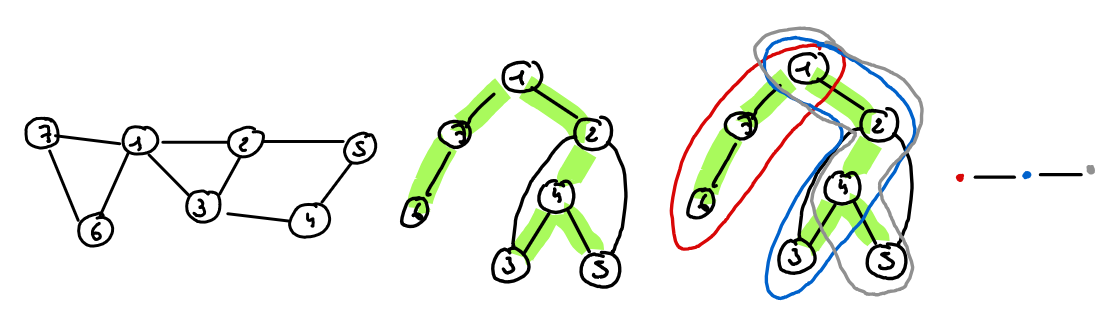
\includegraphics[width=\textwidth]{figures/treedepth-to-pathwidth.png}
    \caption{How to transform an elimination forest into a path decomposition. (a) A graph $G$. (b) An elimination forest of $G$. (c) Bags of a path decomposition of $G$ which follow the elimination forest. (d) The path decomposition of these bags. We can see that the depth of the elimination forest is the same as the width of the path decomposition.}
    \label{fig:treedepth-to-pathwidth}
\end{figure}